%% The first command in your LaTeX source must be the \documentclass command.
%%
%% Options:
%% twocolumn : Two column layout.
%% hf: enable header and footer.
\documentclass[
twocolumn,
% hf,
]{ceurart}

%%
%% One can fix some overfulls
\sloppy

%%
%% Minted listings support 
%% Need pygment <http://pygments.org/> <http://pypi.python.org/pypi/Pygments>
\usepackage{listings}
%% auto break lines
\lstset{breaklines=true}

\usepackage{blindtext}
\usepackage[linesnumbered,ruled]{algorithm2e}
\usepackage{amsmath}
\usepackage{tikzsymbols}
\usepackage{pifont} % for \ding command
\usepackage{listings}
\usepackage{multirow}
\usepackage{bm}
\usepackage{bbm}
\usepackage{xfrac}
\usepackage{booktabs} % For better horizontal rules
\usepackage{cellspace} % For adjusting vertical spacing
\usepackage{xcolor}
\newcommand\todop[1]{\textcolor{red}{#1}} % todo in the paper
\newcommand\todos[1]{\textcolor{blue}{#1}} % todo in the software
\newcommand{\tik}{\textcolor{green}{\ding{51}}}
\newcommand{\ntik}{\textcolor{red}{\ding{55}}}
\usepackage{lastpage}
\usepackage{caption}
\usepackage{subcaption}

\newcommand{\xcc}{\mathbf{x_{/s}}}
\newcommand{\Xcal}{\mathcal{X}}
\newcommand{\xb}{\mathbf{x}}
\newcommand{\xc}{\mathbf{x_c}}
\newcommand{\Xc}{\mathbf{X_c}}
\newcommand{\xci}{\mathbf{x}^i_c}



%%
%% end of the preamble, start of the body of the document source.
\begin{document}

%%
%% Rights management information.
%% CC-BY is default license.
\copyrightyear{2024}
\copyrightclause{Use permitted under Creative Commons License Attribution 4.0 International (CC BY 4.0).}

%%
%% This command is for the conference information
\conference{The 2nd World Conference on eXplainable Artificial Intelligence,
  July 17--19, 2024, Malta, Valetta}

%%
%% The "title" command
\title{RegionalRHALE: A fast and accurate regional effect method for black-box models on tabular data}

%%
%% The "author" command and its associated commands are used to define
%% the authors and their affiliations.
\author[1,2]{Vasilis Gkolemis}
\address[1]{Harokopio University of Athens}
\address[2]{ATHENA Research Center}
\author[1]{Christos Diou}
\author[3]{Eirini Ntoutsi}
\address[3]{University of the Bundeswehr Munich}
\author[2]{Theodore Dalamagas}
% \author[4]{Bernd Bischl}
% \address[4]{Munich Center for Machine Learning (MCML), Department of Statistics, LMU Munich}
% \author[4]{Julia Herbinger}
% \author[4]{Giuseppe Casalicchio}


\begin{abstract}
  The regional effect is a novel explainability method for extracting insights from tabular data through a three-step procedure; a black-box machine learning model is trained on a tabular dataset, a regional effect method explains it and the explanations are used to understand the data and and support decision making.
  Regional effect methods explain the effect of each feature on the ouptput within different subgroups, such as how the age (feature) affects the annual income (output) for men and women separately (subgroups). Identifying meaningful subgroups is computationally intensive, and current regional effect methods face efficiency challenges.
In this paper, we present regional RHALE (r-RHALE), a nover regional effect method designed for enhanced efficiency, making it particularly suitable for decision-making scenarios involving large datasets, i.e., with numerous instances or high dimensionality, and complex models such as deep neural networks. Beyond its efficiency, r-RHALE handles accurately tabular datasets with highly correlated features. We showcase the benefits of r-RHALE through a series of synthetic examples, benchmarking it against other regional effect methods. The accompanying code for the paper is publicly available.
\end{abstract}

%%
%% Keywords. The author(s) should pick words that accurately describe
%% the work being presented. Separate the keywords with commas.
\begin{keywords}
  Explainability \sep
  Interpretability \sep
  Feature Effect \sep
  Regional Effect \sep
  Global Explanations
\end{keywords}

%%
%% This command processes the author and affiliation and title
%% information and builds the first part of the formatted document.
\maketitle


\section{Introduction}
\label{sec:introduction}

Recently, there has been significant progress in Machine Learning (ML) for tabular data, with models capable of learning complex data patterns. Most of these models function as black boxes, meaning their internal workings are not transparent. To address this, eXplainable AI (XAI) has emerged to explain how these models operate. Combining ML with XAI offers a promising approach for data analysis. As illustrated in Figure~\ref{fig:concept_figure}, we can analyze a tabular dataset by explaining a black-box model that is trained on it.

To understand the concept, consider the bike-sharing dataset~\cite{fanaee2014event}. It includes features like temperature, humidity, hour, working/non-working day, and the target variable is the hourly bike-rentals. Suppose a data scientist is hired to analyze this data and help the bike shop owner decide on promotional offers.

The data scientist fits a neural network to the dataset. Then, applies a regional effect method~\cite{herbinger2023decomposing, herbinger_repid_2022} to understand the impact of specific features on the output. The analysis shows that the feature hour is crucial for bike rentals but varies between working days and weekends. On working days (Figure~\ref{subfig:regional_a}), bike rentals spike around 8:30 AM and 5:00 PM because people mainly rent bikes to transport to their work. In contrast, on weekends (Figure~\ref{subfig:regional_b}), rentals rise from 9:00 AM, peak at 12:00 PM, and decline at 4:00 PM, because people mainly rent bikes for sightseeing. 

Based on this analysis, the data scientist advises the bike shop owner to implement promotional offers on differnt hours for working days and weekends. The same analysis can be applied to other features as well.

Unlike global effect methods that provide a single plot per feature, like the global effect of hour on bike-rentals (Figure~\ref{subfig:global}), regional effect methods automatically identify meaningful subregions (e.g., working vs. non-working days). This process is computationally intensive. Current regional effect methods, such as r-PDP, r-ALE, and r-SHAPDP\footnote{The prefix \textit{r-}<name> is a shortcut for \textit{regional-}<name>} becoming slow when the dataset is large (it has many instances) or the black-box model is expensive to evaluate. Additionally, r-PDP struggles when the tabular datahas highly-correlated features, where it may identify incorrect subregions due to out-of-distribution sampling.

To address these challenges, we introduce r-RHALE, a regional effect method built on RHALE~\cite{gkolemis2023rhale, gkolemis22a}, which:

\begin{itemize}
\item is efficient, making it suitable for datasets with numerous instances and expensive black-box models, such as deep neural networks.
\item effectively handles cases with correlated features, avoiding out-of-distribution sampling.
\end{itemize}

We demonstrate these advantages with two synthetic examples. The code for reproducing the results is publicly available.

\begin{figure*}[t]
    \centering
    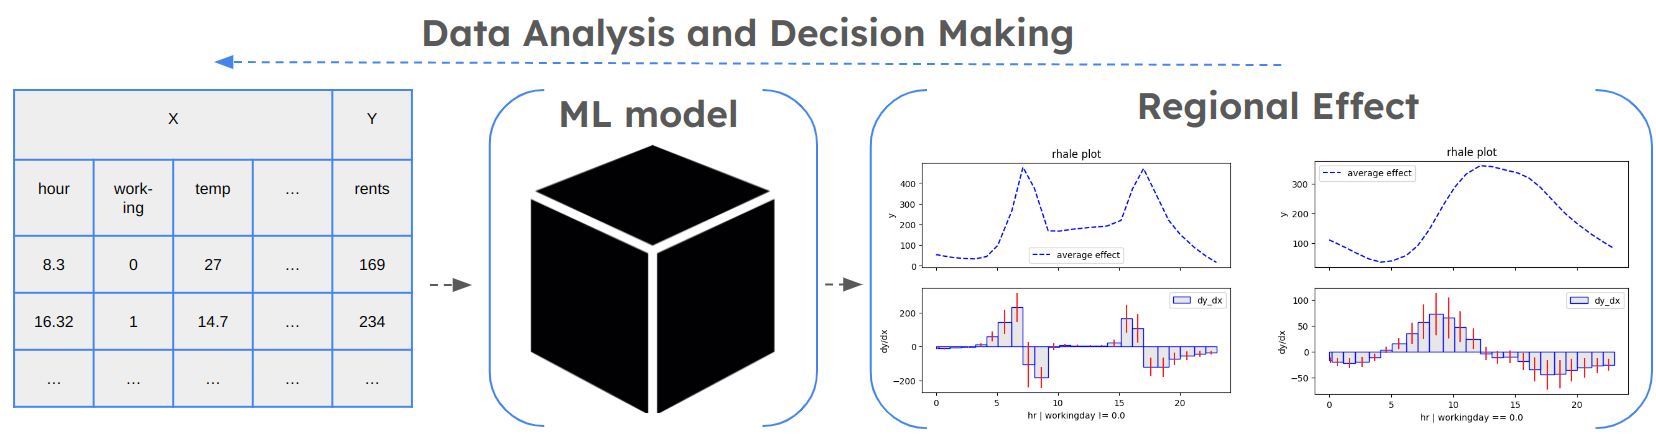
\includegraphics[width=\textwidth]{figures/concept_image.png}
    \caption{Data analysis and decision making pipeline: Utilizing regional effect plots to extract insights from tabular data.}
    \label{fig:concept_figure}
\end{figure*}

\section{Regional RHALE}


r-RHALE is the regional version of RHALE, a global effect method for differentiable black-box models. It builds on two key papers. The first, by Gkolemis et al. (2023)~\citep{gkolemis2023rhale}, introduced RHALE, a faster version of ALE which also computes the heterogeneity, an important quantity for subregion detection. The second paper, by Herbinger et al. (2023)~\citep{herbinger2023decomposing}, proposed a generic framework for transforming global effect methods to regional and applied it to PDP, ALE, and SHAP-DP.


\begin{figure*}
  \centering
  \begin{subfigure}[t]{0.32\textwidth}
  \centering
  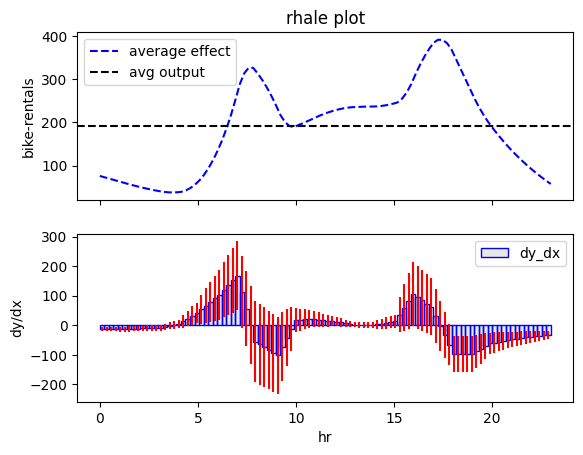
\includegraphics[width=\linewidth]{figures/running_example/01_bike_sharing_dataset_23_1.png}
  \caption{Global effect}
  \label{subfig:global}
  \end{subfigure}
  \begin{subfigure}[t]{0.32\textwidth}
  \centering
  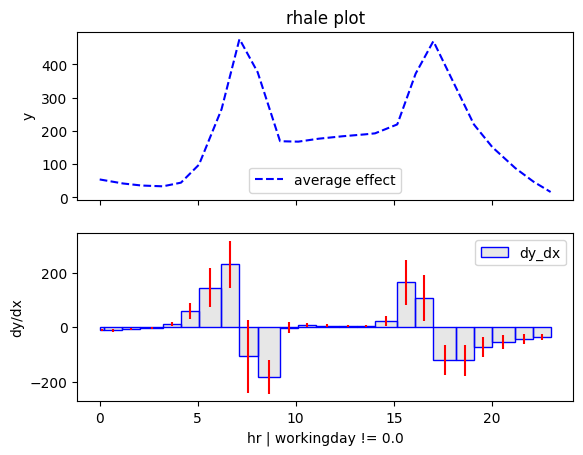
\includegraphics[width=\linewidth]{figures/running_example/01_bike_sharing_dataset_29_1.png}
  \caption{Regional on working days}
  \label{subfig:regional_a}
  \end{subfigure}
  \begin{subfigure}[t]{0.32\textwidth}
  \centering  
  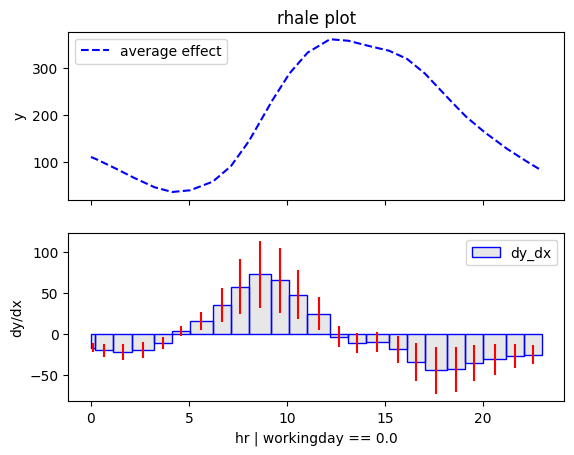
\includegraphics[width=\linewidth]{figures/running_example/01_bike_sharing_dataset_29_0.png}
  \caption{Regional on non-working days}
  \label{subfig:regional_b}
  \end{subfigure}
  \caption{\texttt{RegionalPDP} applied to the Bike Sharing dataset; Left: Global effect of feature \texttt{hour} on the \texttt{bike-rentals}. Middle: Regional effect of feature \texttt{hour} on weekdays. Right: Regional effect of feature \texttt{hour} on weekends.}
  \label{fig:main-concept}
\end{figure*}

\subsection{Method Description}

\paragraph{Notation.}

Let \(\mathcal{X} \in \mathbb{R}^d\) be the \(d\)-dimensional feature space, \(\mathcal{Y}\) the target space and
\(f(\cdot) : \mathcal{X} \rightarrow \mathcal{Y}\) the black-box function.
We use index \(\mathtt{s} \in \{1, \ldots, d\}\) for the feature of interest and \(\mathtt{C} = \{1, \ldots, d\} - s\) for the indices of all the other features.
For convenience, we use \((x_s, \xc)\) to denote the input vector \((x_1, \cdots , x_s, \cdots, x_D)\),
\((X_s, \Xc)\) instead of \((X_1, \cdots , X_s, \cdots, X_D)\) for random variables and
$\mathcal{X}_s, \mathcal{X}_{c}$ for the feature space and its complement, respectively.
The training set \(\mathcal{D} = \{(\xb^i, y^i)\}_{i=1}^N\) is sampled
i.i.d.\ from the distribution \(\mathbb{P}_{X,Y}\).

\paragraph{RHALE global effect.}

RHALE esitmates the effect of feature $x_s$ on the output $y$ (Figure~\ref{fig:concept_figure} - right), with the following formula:

\begin{equation}
  \label{eq:rhale-approximation}
\hat{f}^{\mathtt{RHALE}}(x_s) = \sum_{k=1}^{k_{x_s}} \underbrace{\frac{z_k - z_{k-1}}{ \left | \mathcal{S}_k \right |} \sum_{i: \xb^i \in \mathcal{S}_k} \frac{\partial f}{\partial x_s} (x_s^i, \xci)}_{\hat{\mu}_k^{\mathtt{RHALE}}}
\end{equation}

\noindent
The axis of feature $x_s$ is partitioned into a sequence of $K_s$ variable-size intervals, i.e., $\{\mathcal{Z}_k\}_{k=1}^{K_s}$, where each interval covers the range $[z_{k-1}, z_k)$. We denote $\mathcal{S}_k$ the set of instances with the $s$-th feature inside the $k-$th interval, i.e., $\mathcal{S}_k = \{ x^{(i)} : z_{k-1} \leq x^{(i)}_s < z_k \}$. The limits of the intervals is computed by solving an optimization problem as described in~\citep{gkolemis2023rhale}.

\paragraph{Intuition.} $\frac{\partial f}{\partial x_s} (x_s^i, \xci)$ is the effect of the $s$-th feature computed on the $i$-th instance. It shows the change on the output, if we slightly change the instance from $(x_s^i, \xci)$ to $(x_s^i + \delta, \xci)$. Then we average the local effects from all instances that lie inside the $k$-th bin, getting the average bin effect, $\hat{\mu}_k^{\mathtt{RHALE}} = \frac{z_k - z_{k-1}}{ \left | \mathcal{S}_k \right |} \sum_{i: \xb^i \in \mathcal{S}_k} \frac{\partial f}{\partial x_s} (x_s^i, \xci)$. Finally, we sum the bin effects to compute the curve of Figure.

\paragraph{Heterogeneity}

The heterogeneity is a number that shows to what extent the local effects deviate from the average effect. In RHALE it is defined as:

\begin{equation}
  \label{eq:rhale-approximation-heterogeneity}
  \hat{H}_s^{\mathtt{RHALE}} = \sum_{k=1}^{K_s} \frac{z_k - z_{k-1}}{|\mathcal{S}_k|}\sum_{i: \xb^i \in \mathcal{S}_k} \left [ \frac{\partial f}{\partial x_s} (x_s^i, \xci) - \hat{\mu}_k^{\mathtt{RHALE}} \right ]^2
\end{equation}

\noindent
Zero heterogeneity means that effect of $x_s$ on the output does not depend on any other feature, i.e., that $f(\xb)$ can be written as $f_c(\xc) + f_s(x_s)$. In other cases, the heterogeneity is positive and larger heterogeneity means stronger dependence on one or more features in $/s$. 

\paragraph{Regional RHALE}

r-RHALE is the combination of the heterogeneity as defined in Eq.~(\ref{eq:rhale-approximation-heterogeneity}) and the CART-based algorithm of all regional effect approaches that is analyzed as detailed in~\cite{herbinger2023decomposing, gkolemis2024effector}. Here, we will provide an intuitive explanation of how it works and highlight its computational advantages.

Regional effect methods search for subregions that minimize heterogeneity. This means that within these subregions, the effect of a feature \( x_s \) on the output is less influenced by the values of other features. A subregion is defined by conditioning on another feature \( x_c \); for continuous features, the condition is whether the feature value is greater or less than a threshold, i.e., \( \tau \), and for categorical features, whether it equals or differs from \( \tau \). The CART-based algorithm that searches for these regions iterates over all features in \( \xb_c \) and tests splits at various positions \( \tau \) to identify the split that results in the greatest reduction in heterogeneity.

The computational advantage of r-RHALE over other methods lies in its definition of heterogeneity. According to Eq.~(\ref{eq:rhale-approximation-heterogeneity}), the term \( \frac{\partial f}{\partial x_s} (x_s^i, \xci) \) needs to be computed only once for all instances. If the method runs in a batched fashion and supports automatic differentiation, the execution time is comparable to a single evaluation of \( f \). In contrast, other approaches must re-evaluate \( f \) multiple times to obtain regional effects, leading to slower execution times, especially when \( f \) is complex and computationally intensive.

\section{Synthetic Examples}

We create and test our approach on two synthetic examples. The synthetic example of Section~\ref{sec:efficiency} demonstrates that r-RHALE is faster than the existing methods and the example of Section~\ref{sec:correlated-features}, unlike r-PDP, it handles well tabular datasets with correlated features.

\subsection{Execution time comparison}
\label{sec:efficiency}


In this example, we show that r-RHALE executes significantly faster than r-PDP and r-ALE.
We do not include r-SHAPDP in the comparison, because its execution time is prohibitive high, e.g., more than 30 minutes, even for relatively light models and datasets. In the example, we observe that r-RHALE executes fast even under a (a) slow-inference black-box model and (b) a large tabular dataset.

\paragraph{Slow-inference black-box model:}

We generate a synthetic dataset with $N=10^4$ instances and $D=10$ features. Then, we train deep neural networks (DNN) with number of layers ranging from $L=3$ to $L=20$. The only factor that a larger neural network affects is the inference time, so our findings generalize to all black-box models with slow inference.

In Figure~\ref{fig:efficiency_heavy_model}, we observe that r-RHALE execution time increases at a much slower rate compared to r-ALE and r-PDP. Consequently, even for a complex model, such as a deep neural network (DNN) with 20 layers, r-RHALE requires less than 15 seconds to generate regional effect plots for a single feature. This translates to approximately 4-5 minutes for a typical tabular dataset with around 20 features. In contrast, r-PDP requires about 4 minutes per feature, totaling approximately an hour for all features, while r-ALE needs about 1 minute per feature, resulting in roughly 20 minutes for all features.

\begin{figure}
    \centering
    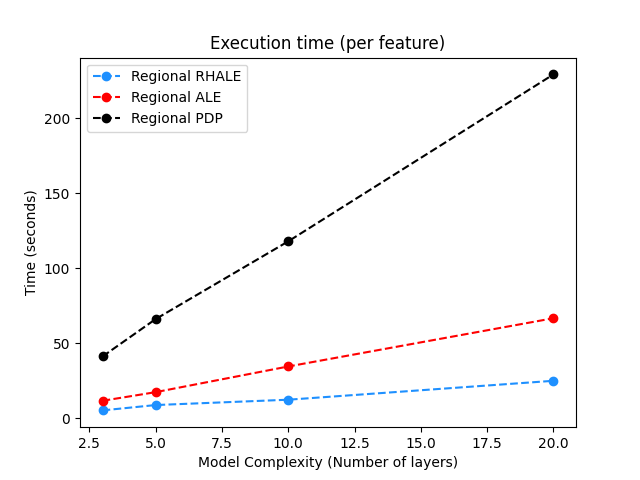
\includegraphics[width=.49\textwidth]{figures/simulation_2/efficiency_layers.png}
    \caption{Execution time of regional effect methods applied on a neural network with a varying number of layers. More layers indicate a black-box model with longer inference times.}
    \label{fig:efficiency_heavy_model}
\end{figure}

\paragraph{Large tabular dataset:}

We create a deep neural network (DNN) with \( L = 5 \) layers and generate a synthetic dataset with \( D = 20 \) features and a varying number of instances \( N \in \{10^3, 10^4, 10^5\} \) (log scale).

In Figure~\ref{fig:efficiency_nof_instances}, we observe that r-RHALE is the fastest approach as the number of instances increases. r-RHALE is more than twice as fast as r-ALE and ten times faster than r-PDP. For large datasets, this translates to a speed-up of 20 minutes compared to r-ALE and 2 hours compared to r-PDP. The efficiency gain would be even more pronounced with a heavier black-box model, as demonstrated in the previous example.

\begin{figure}
    \centering
    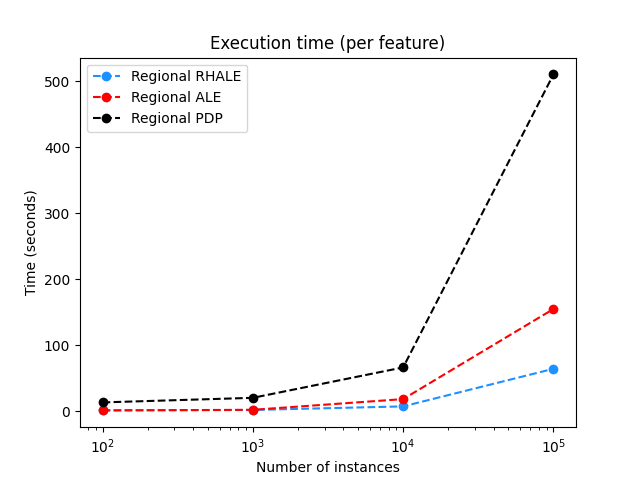
\includegraphics[width=.49\textwidth]{figures/simulation_2/efficiency_samples.png}
    \caption{Data analysis and decision making pipeline: Utilizing regional effect plots to extract insights from tabular data.}
    \label{fig:efficiency_nof_instances}
\end{figure}


\subsection{Correlated Features}
\label{sec:correlated-features}

In this example, we demonstrate that r-RHALE effectively handles cases with correlated features, while r-PDP may incorrectly identify subregions due to out-of-distribution sampling.

We use the model \( y = 3x_1I_{x_3 > 0} - 3x_1I_{x_3 \leq 0} + x_3 \) with two different data-generating distributions. In the non-correlated setting, all variables are uniformly distributed, \( x_i \sim \mathcal{U}(-1,1) \). In the correlated setting, \( x_1 \) and \( x_2 \) maintain the same distributions, but \( x_3 = x_1 \).

These two versions illustrate that r-PDP produces the same regional effect regardless of correlations, while r-RHALE accurately distinguishes between the two cases. We focus on the effect (both global and regional) of \( x_1 \) on \( y \).

\paragraph{Non-correlated setting.}

The effect of \( x_1 \) arises from the interaction terms \( 3x_1I_{x_3>0} \) and \( 3x_1I_{x_3\leq0} \). The global effect will be \( 3x_1 \) when \( x_3 > 0 \) (half the time, given \( x_3 \sim \mathcal{U}(-1,1) \)) and \( -3x_1 \) when \( x_3 \leq 0 \) (the other half). This results in an overall zero global effect with high heterogeneity. By splitting into two subregions, \( x_3 > 0 \) and \( x_3 \leq 0 \), we obtain two regional effects, \( 3x_1 \) and \( -3x_1 \), each with zero heterogeneity.

In Figure~\ref{fig:synthetic-1-uncorrelated}, both r-PDP and r-RHALE correctly identify the global effect. The global effect is zero but with high heterogeneity, indicated by the two red lines in the r-PDP plot (Figure~\ref{subfig:global_pdp}) and the red bars in the r-RHALE plot (Figure~\ref{subfig:global_rhale}). Due to space limitations, we do not illustrate the regional effects, which, in both cases, match the ground truth.

\begin{figure}[t]
    \centering
    \begin{subfigure}[b]{0.24\textwidth}
        \centering
        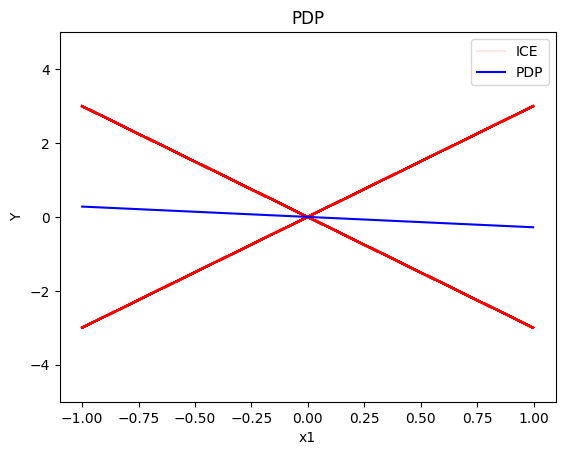
\includegraphics[width=\textwidth]{figures/simulation_1/uncor_global_pdp.png}
        \caption{Global PDP ($x_1$)}
        \label{subfig:global_pdp}
    \end{subfigure}
    \begin{subfigure}[b]{0.24\textwidth}
        \centering
        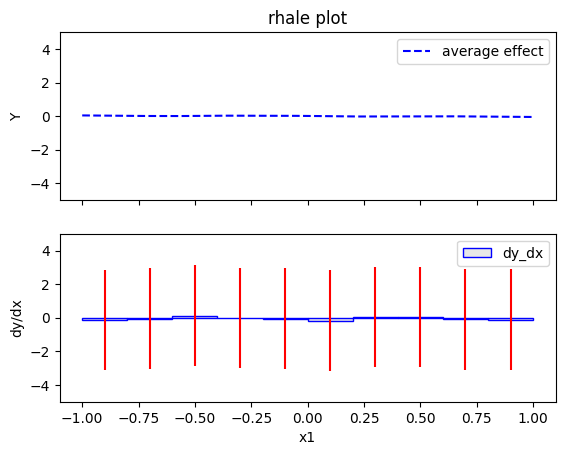
\includegraphics[width=\textwidth]{figures/simulation_1/uncor_global_rhale.png}
        \caption{Global RHALE ($x_1$)}
        \label{subfig:global_rhale}
    \end{subfigure}
    \caption{Global plots for the non-correlated setting using PDP and RHALE methods.}
    \label{fig:synthetic-1-uncorrelated}
  \end{figure}

\paragraph{Correlated setting.}

In the correlated case, with \( x_3 = x_1 \), the effect becomes \( y = 3x_1I_{x_1 > 0} - 3x_1I_{x_1 \leq 0} \). This is because the interaction terms simplify to \( 3x_1I_{x_1 > 0} \) and \( -3x_1I_{x_1 \leq 0} \). When \( x_1 > 0 \), \( x_3 > 0 \), so only the \( 3x_1 \) term is active. Similarly, when \( x_1 \leq 0 \), \( x_3 \leq 0 \), making only the \( -3x_1 \) term active.

In Figure~\ref{fig:synthetic-1-correlated}, we observe that only r-RHALE correctly estimates the global and regional effects. r-RHALE (Figure~\ref{subfig:global_rhale_correlated}) accurately computes the effect as \( 3x_1I_{x_1 > 0} - 3x_1I_{x_1 \leq 0} \) with no heterogeneity and does not identify subregions. In contrast, r-PDP (Figure~\ref{subfig:global_pdp_correlated}) treats the features as independent, resulting in the same global effect as in the uncorrelated case and incorrectly identifying subregions for \( x_3 > 0 \) and \( x_3 \leq 0 \).


\begin{figure}[t]
    \centering
    \begin{subfigure}[b]{0.24\textwidth}
        \centering
        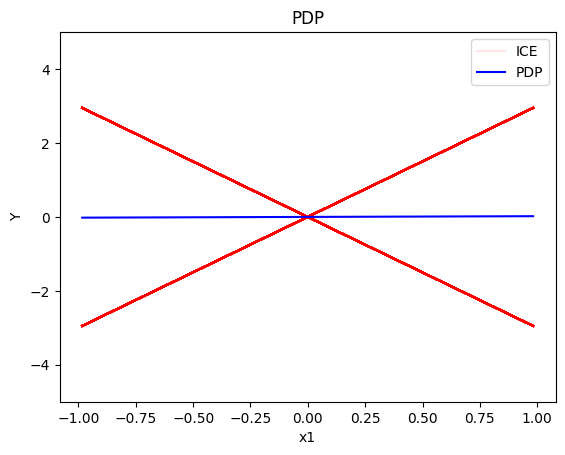
\includegraphics[width=\textwidth]{figures/simulation_1/cor_global_pdp.png}
        \caption{Global effect}
        \label{subfig:global_pdp_correlated}
    \end{subfigure}
    \begin{subfigure}[b]{0.24\textwidth}
        \centering
        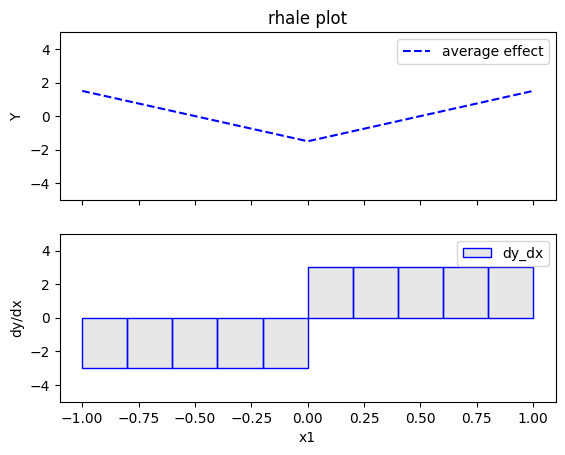
\includegraphics[width=\textwidth]{figures/simulation_1/cor_global_rhale.png}
        \caption{Global effect}
        \label{subfig:global_rhale_correlated}
    \end{subfigure}
    \caption{Global plots for the correlated setting using PDP and RHALE methods.}
    \label{fig:synthetic-1-correlated}
  \end{figure}
  
  
\section{Conclusion and Future Work}

In this paper, we introduce a novel method for extracting insights from tabular data. Our approach involves first fitting a black-box model and then explaining its predictions using a regional effect method. The insights gained from the regional effect can then be applied to support decision-making processes.

To this end, we propose r-RHALE, an innovative regional effect method that builds upon the strengths of the global effect RHALE. r-RHALE offers significantly improved efficiency compared to existing methods and effectively handles datasets with correlated features.

\bibliography{regional_rhale.bib}

\end{document}

%%
%% End of file
